\section{Experiment and Results} 

\subsection{Implementation details} 

For CP-VTON+ network implementation is based on CP-VTON PyTorch and extended the network as described above. We also used the modified human image segmentation and human representation. The network  For training, we refer \cite{Wang2018TowardCI} and used similar setting for comparison. We used $L_1 = L_{vgg} = L_{mask} =1$ and $L_{reg} = 0.5$ through  hyper-parameter tuning. We trained both networks for 200K steps with batch size 4 with Adam optimizer with $\beta_1 = 0.5$ and $\beta_2 = 0.999$. Learning rate is first fixed at $0.0001$ for 100K steps and then linearly decays to zero for the remaining steps. 

\subsection{Comparative Results}

To evaluate the performance improvement of CP-VTON+, we compare the performance with CP-VTON, since CP-VTON shows the best performance in the previous research and our in-depth comparison study.

VITON cloth-human pair dataset is again used for training and test dataset. We used IoU and SSIM performance metrics for the same cloth retry-on cases for warping stage and blending stage, respectively. The original target human image is used for the reference image for SSIM and the parsed segmentation area for the current top cloth is used for IoU reference. Our proposed method, CP-VTON+ outperforms CP-VTON all measures: in IoU  with  0.8325 over o.7883 (around 7 $\%$)and in SSIM with 0.8163 over 0.7798 (around 5 $\%$). The performance improvement in warping stage is lager than final results. 
Since SSIM is originally developed for geometrically aligned image comparison, Learned Perceptual Image Patch Similarity (LPIPS) metric \cite{zhang2018unreasonable} measure is added to evaluate the deep learning visual similarity. CP-VTON+ outperforms CP-VTON in LPIPS with 0.1263 over 0.1397.

% TODO check smaller is better???


%Special comments are required for the IoU values, where CP-VTON (0.78) is slightly higher than CP-VTON+ (0.75). The un-expected results originated due to CP-VTON generating as in the current cloth shape. However, similar clothes are not always applicable, furthermore, it generates wrong shaped results for different clothes. Fig. 6 illustrates this with two typical example, plugging and normal tops

For different cloth try-on, Inception Score (IS) is used together with visual examinations. CP-VTON+ outperforms slightly CP-VTON in IS with 2.76 over 2.7417. Figure \ref{fig:2dvton_same} and Figure \ref{fig:2dvton_diff} show the representative results selected for presentation. The subjective evaluation shows significant visual improvements.  1) the warped clothes do not have severe distortion. 2) the bottom clothes are retained. 3) the new cloth collar shape is not affected by the current cloth's collar shape. 4) cloth textures such as logos and patterns are clearer.
 
 
%We added the test results for all test cases for comparison between CP-VTON and CP-VTON+ in supplementary materials, together with the categorized comparison of SCM-based VTON, VITON and CP-VTON

%\begin{figure}
%\centering
%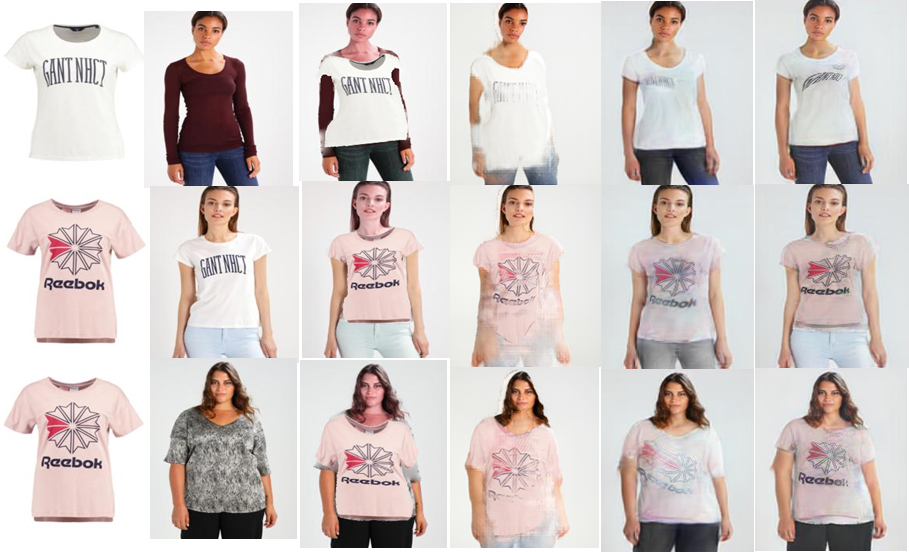
\includegraphics[height=6.5cm, scale=1]{figures/cpvton+compare.png} 
%\caption{VTON results: We have to include 1) %GMM and TOM results for demonstrating all the improvement one by one: }
%\label{fig:vtonresults}
%\end{figure}


\subsection{Ablation Study}

Figure ~\ref{fig:ablation} we highlight the impact of the identified problems and improvement of the proposed method step-by-step through the ablation study of CP-VTON+. The first and second columns are target humans and try-on clothes, respectively. The third column is vanilla CP-VTON results. The fourth column is when unchanged clothes and body parts are added to the reserved region inputs of TOM, retaining the original pants texture. The fifth column is when the mask loss function of TOM is updated with the target cloth area, making the texture and color of cloth sharp and vivid. Finally the sixth and last column is when the body masks are updated, replacing the skin area wrongly labelled as background and hair are removed from the reserved region input of GMM, making GMM can better cloth-and-hair-agnostic human representation.  


\begin{figure}[t]
\centering
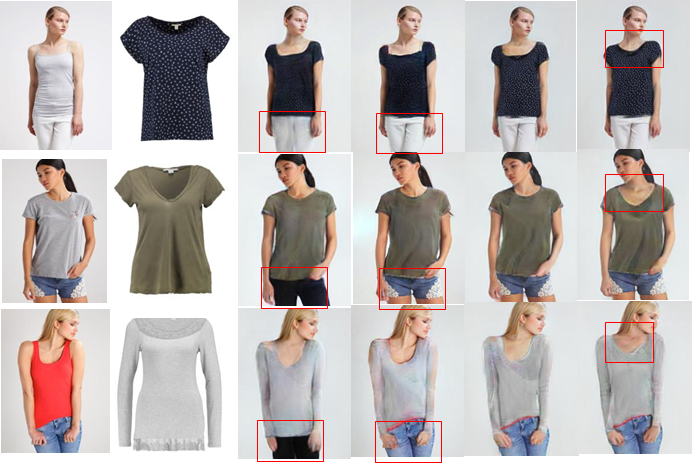
\includegraphics[height=6.5cm, scale=1]{figures/ablation.png} 
\caption{Ablation study of CP-VTON+. From left to right column: target humans, try-on clothes, CP-VTON, with corrected human representation in TOM, warped cloth mask and mask loss function updated, and CP-VTON+ (with corrected human representation in GMM)
}
\label{fig:ablation}
\end{figure}


\subsection{Discussion}

Even though CP-VTON+ improves the quality to some degree, and showing highly natural results, the experiment is still limited because the dataset has limited samples for difficult cases, like the long sleeved, complicated shaped, or textured cloth and large posture target human. 

As Figure ~\ref{fig:gmmfailure} shows two typical failure cases due to the cloth warping. First row shows when the arms heavily covers the body area. The warped cloth does not match to the human body and TON failed in hiding the warping error. 
% STN (Spatial Transform Network). STN is originally developed for invert the (augmented) input images for different camera views and camera distortion.
Any classical 2D transform including on-rigid TPS algorithms, cannot handle the strong 3D deformations of cloth.  Also the 3D poses induce self-occlusions. The TON network should recognized the cloth area and skin areas, like naked arms. One practical short-term solution would be to restrict the pose of target human image from the customer. 

The second rows shows the another problems. Even without strong 3D posture of the target human, the warped cloth often shows un-realistic results. Note that even though the CNN geometric matching argues it can cover the category-level matching. The category is not precisely defined for our application. Mostly the cloth texture can not be used for image feature and the cloth-agnostic human representation does not have even any texture information. Note that the matching algorithm is in fact used without in-depth study on the accuracy for VTON applications. 

    
The output image quality of all image-based VTON algorithms including ours depend upon the quality of input human representation, i.e., estimated joint locations and parsed human segmentation. The poses of target humans are usually (or forced) rather simple so that the state-of-the-art pose estimation algorithms can provide fairly accurate positions. However the quality of parsed human are not always good enough, especially when the target human wear complicated clothes. Also one can restrict the complexity of human images in pose and cloth style, but still the accuracy at the segmentation boundary sometimes affects the blended image results as shown in third row case in Figure ~\ref{fig:ablation}, where the pixels of the current top cloth, which is mislabelled as bottom cloth, remained in the blending result. There fore high quality human parsing algorithm especially around boundaries are required.   

\begin{figure}
\centering
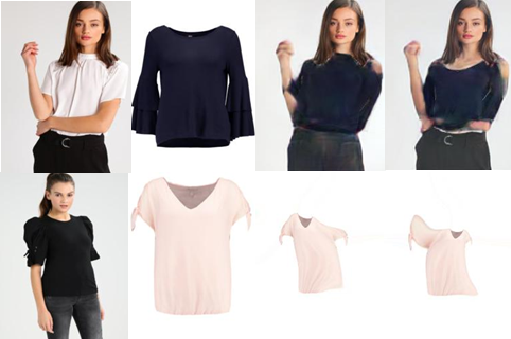
\includegraphics[height=4.5cm, scale=1]{figures/gmmfailure.png} 
\caption{Cloth Warping Failure of CP-VTON+. From left to right column. target humans, try-on clothes, CP-VTON, and CP-VTON+  (Why not same first and second ??)
}
\label{fig:gmmfailure}
\end{figure}
 